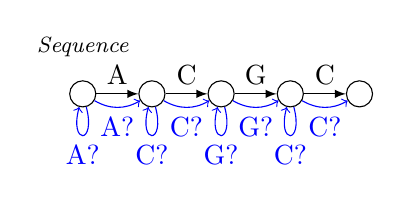
\begin{tikzpicture}[auto]
	\tikzstyle{state} = [ draw, circle, thin, node distance = 2.5em, font={\small}];
	\tikzstyle{query} = [ draw, rectangle, thin, node distance = 2.5em, font={\small}];
	\tikzstyle{info} = [font={\itshape\footnotesize}]
	\tikzstyle{point}  = [ ->, thin, font={\small}];
	\tikzstyle{extend} = [ ->, double, font={\small}];
	\tikzstyle{trace} = [ ->, thick, dashed, bend right, font={\small} ];


	\def \seq {X,A,C,G,C}

	\foreach \x [count=\xi] in \seq {
		\ifnum 1 < \xi
			\pgfmathparse{int(\xi-1)}
			\let \li \pgfmathresult
			\node[state, right of=\li] (\xi) {};
			\draw[->, >=latex] (\li) to node{\x} (\xi);
		\else
			\node[state] (\xi) {};
		\fi
	}

	\node[info] at (0,0.6) {Sequence};

    \tikzstyle{starQ} = [->, thin, color=blue ];

	\foreach \x [count=\xi] in \seq {
		\ifnum 1 < \xi
			\pgfmathparse{int(\xi-1)}
			\let \li \pgfmathresult
			\draw[starQ, bend right] (\li) to node[below]{\x?} (\xi);
			\draw[starQ, loop below] (\li) to node{\x?} (\li);
		\else
		\fi
	}
\end{tikzpicture}
